%! Author = Raffaele Talente
%! Date = 16/01/2024

% Preamble
\documentclass[11pt,italian,a4paper,oneside,openright]{article}

% Packages
\usepackage{amsmath}
\usepackage{graphicx}
\usepackage[hyperindex]{hyperref}
\usepackage{amsfonts}
\usepackage{vmargin}
\usepackage{ragged2e}

\graphicspath{{img/}}
\hypersetup{colorlinks=true, linkcolor=black}

\title{Network Pong}
\author{Raffaele Talente}

% Document
\begin{document}
    \pagenumbering{Roman}
    \vskip 1cm \large \centerline{\textsc{Università degli Studi di
    Napoli ``Parthenope''}}

    \centerline {\small\textsc{Corso di laurea in Informatica
        (percorso Generale)}}

    \begin{center}
        
\includegraphics[scale=0.24]{logo_parthenope}
    \end{center}

    \vskip 0.5cm

    \large \centerline {\textsc{Corso di Reti di Calcolatori e Laboratorio}}

    \vskip 0.5cm

    \Large \centerline {Network Pong}


    \vskip 4.5cm


    \large
    \begin{minipage}[t]{7cm}
        \textsc{Docente}

        Emanuel Di Nardo\\

    \end{minipage}
    \hfill
    \begin{minipage}[t]{5cm}
        \hfill \textsc{Candidato}

        \hfill Raffaele Talente
        \hfill 0124002658
    \end{minipage}

    \vskip 2.0 cm \Large \centerline {Anno Accademico 2023--2024}
    \vfill \eject

    \tableofcontents

    \newpage

    \pagenumbering{arabic}
    %! Author = Raffaele
%! Date = 16/01/2024

\newpage
\thispagestyle{headings}
\section{Descrizione del progetto}\label{sec:Descrizione}
L'obiettivo del progetto è quello di implementare un gioco basato su \textbf{Pong},
tramite comunicazione in tempo reale con UDP. \\
Pong, uno dei primissimi videogiochi arcade, è un simulatore di ping-pong bidimensionale:
i due giocatori controllano una racchetta ciascuno, situate ai due lati dello schermo,
e si scambiano una pallina che si muove da un lato all'altro dello schermo.
Nel momento in cui un giocatore non riesce a intercettare la pallina l'avversario guadagna un punto. \\

Il progetto è stato sviluppato utilizzando il linguaggio di programmazione \textbf{Python}.
La griglia di gioco è stata rappresentata come una griglia di caratteri, che possono essere vuoti,
occupati da una racchetta oppure occupati dalla pallina.
E' stata inoltre utilizzata la libreria \textbf{Pygame} per gestire l'input da tastiera dell'utente
e la rappresentazione a schermo della griglia di gioco.
    %! Author = Raffaele
%! Date = 17/01/2024

\newpage
\thispagestyle{headings}
\section{Schema dell'architettura}\label{sec:Schema}
L'architettura del progetto è basata su una rete P2P puramente decentralizzata, in quanto
tutti i nodi sono uguali, sebbene quantitativamente piccola: \\
I due giocatori costituiscono i \textbf{Peer}, poiché svolgono la funzione sia di
client che di server: entrambi devono notificare immediatamente la controparte riguardo
i movimenti della propria racchetta, inoltre l'ultimo giocatore che ha toccato la pallina deve fare
da \textit{seeder}, deve cioè calcolare il movimento della pallina e comunicarlo alla controparte.
Il seeder si occupa anche di aggiornare il punteggio e di comunicarlo all'altro giocatore.

\begin{figure}
    \centering
    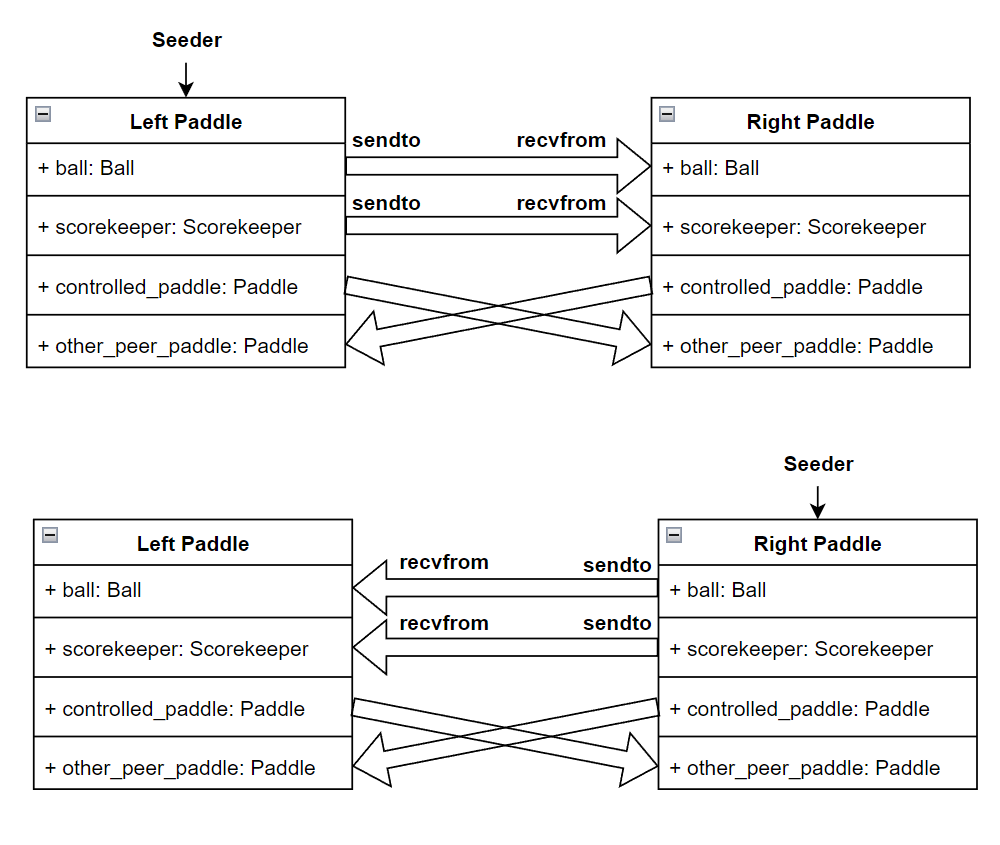
\includegraphics[scale=0.5]{img/schema}
    \caption{Schema dell'architettura}
    \label{fig:schema}
\end{figure}


    %! Author = Raffaele
%! Date = 17/01/2024

\thispagestyle{headings}
\newpage
\section{Dettagli implementativi}\label{sec:implementazione}

\subsection{Implementazione dei Peer}\label{subsec:implementazione-dei-peer}

La classe Peer è stata progettata nel seguente modo:
\begin{itemize}
    \item Il costruttore della classe crea la socket UDP ed effettua il bind su tutte le interfacce, utilizzando
    una porta di default arbitaria. \\
    Vengono poi create le variabili degli oggetti utilizzati all'interno del gioco, l'implementazione
    delle classi di tali oggetti è presente nel file
    \textit{app/components.py}.
    \item L'indirizzo dell'altro peer viene passato come argomento da linea di comando ed inserito opportunamente.
    \item Il metodo send\_data trasforma l'oggetto Python da inviare in uno stream di byte attraverso il modulo
    \textit{pickle}.
    \item Il metodo \textit{receive\_data} gestisce l'ottenimento dei dati dalla \textit{recvfrom}, trasformando lo
    stream di byte in un oggetto Python. \\
    E' importante inserire un timeout, in quanto è imperativo che la recvfrom non blocchi indefinitivamente il processo:
    il timeout è stato impostato tramite una costante a \textit{5.5 ms}, questo numero deriva dal fatto che se si vuole
    mantenere il gioco a 60 \textit{frame al secondo}, è necessario che ogni frame non richieda più di \textit{16.6 ms}.
    Poiché in ogni frame un Peer al più deve ricevere informazioni sulla pallina, sulla racchetta dell'altro giocatore
    e sullo score, il valore massimo di attesa non può essere più elevato.
    \item Il metodo \textit{receive\_and\_replace\_object\_data} richiama il metodo \textit{receive\_data} ed effettua
    l'azione appropriata a seconda dell'oggetto ritornato.
        \begin{itemize}
            \item Se viene ritornato un oggetto, si aggiorna opportunamente la variabile relativa.
            \item Se la chiamata va in \textit{timeout}, la funzione ritorna. \\
            Il timeout viene effettivamente ignorato in quanto è importante che il gioco prosegui, uno spostamento
            di un frame mancato non è particolarmente impattante sull'applicazione rispetto ad un processo che si blocca
            per assicurarsi che ogni pacchetto inviato sia ricevuto.
            \item Se vi è un altro errore, solitamente causato dalla mancanza dell'altro peer, il processo semplicemente
            va in sleep per un secondo prima di ritentare.
        \end{itemize}
\end{itemize}

\begin{figure}
    \begin{verbatim}
    # import omessi per semplicità

        class Peer:
    def __init__(self, paddle_id):
        # viene creata una socket associata al peer
        # il bind viene effettuato su '', che è l'equivalente di INADDR_ANY
        self.peer_socket = socket.socket(socket.AF_INET, socket.SOCK_DGRAM)

        # come porta viene utilizzata una porta di default arbitaria
        # a cui viene aggiunto l'id del paddle
        self.peer_socket.bind(('', DEFAULT_PORT + paddle_id))

        # l'id è 0 (racchetta sinistra) o 1 (racchetta destra)
        self.id = paddle_id

        # inizializzazione delle variabili utilizzate dalla classe
        self.other_peer = ('', DEFAULT_PORT + paddle_id)
        self.controlled_paddle = Paddle()
        self.other_peer_paddle = Paddle()
        self.ball = Ball()
        self.scorekeeper = Scorekeeper()

    # l'indirizzo dell'altro seed viene passato
    # come argomento da riga di comando
    def set_other_peer(self, address):
        if self.id == LEFT_PADDLE_ID:
            self.other_peer = (address, DEFAULT_PORT + RIGHT_PADDLE_ID)
        else:
            self.other_peer = (address, DEFAULT_PORT + LEFT_PADDLE_ID)
    \end{verbatim}
    \caption{Implementazione del costruttore della classe Peer}
    \label{fig:peer1}
\end{figure}

\begin{figure}
    \begin{verbatim}
    # invia dati all'altro peer
    # trasforma l'oggetto in uno stream di byte con pickle
    def send_data(self, object_data):
        data = pickle.dumps(object_data)
        self.peer_socket.sendto(data, self.other_peer)

    # riceve dati dall'altro peer dopo aver inserito il timeout
    # ritorna un oggetto Python ottenuto dallo stream di byte con pickle
    def receive_data(self):
        self.peer_socket.settimeout(TIMEOUT)
        data, address = self.peer_socket.recvfrom(MAX_BUF)
        object_data = pickle.loads(data)
        return object_data

    # ottiene un oggetto chiamando il metodo receive_data
    # ed effettua l'operazione appropriata
    def receive_and_replace_object_data(self):
        object_data = object
        try:
            object_data = self.receive_data()

        # se la recvfrom va in timeout la funzione semplicemente ritorna
        except socket.timeout:
            return

        # se l'altro processo non è presente, aspetta
        except socket.error:
            print('waiting for the other peer...')
            time.sleep(1)

        # se riceve un oggetto correttamente
        # effettua l'operazione appropriata
        if type(object_data) is Ball:
            self.ball = object_data
        elif type(object_data) is Paddle:
            self.other_peer_paddle = object_data
        elif type(object_data) is Scorekeeper:
            self.scorekeeper = object_data
    \end{verbatim}
    \label{fig:peer2}
\end{figure}


    %! Author = Raffaele
%! Date = 17/01/2024

\newpage
\section{Il gioco}\label{sec:gioco}

\begin{figure}
    \centering
    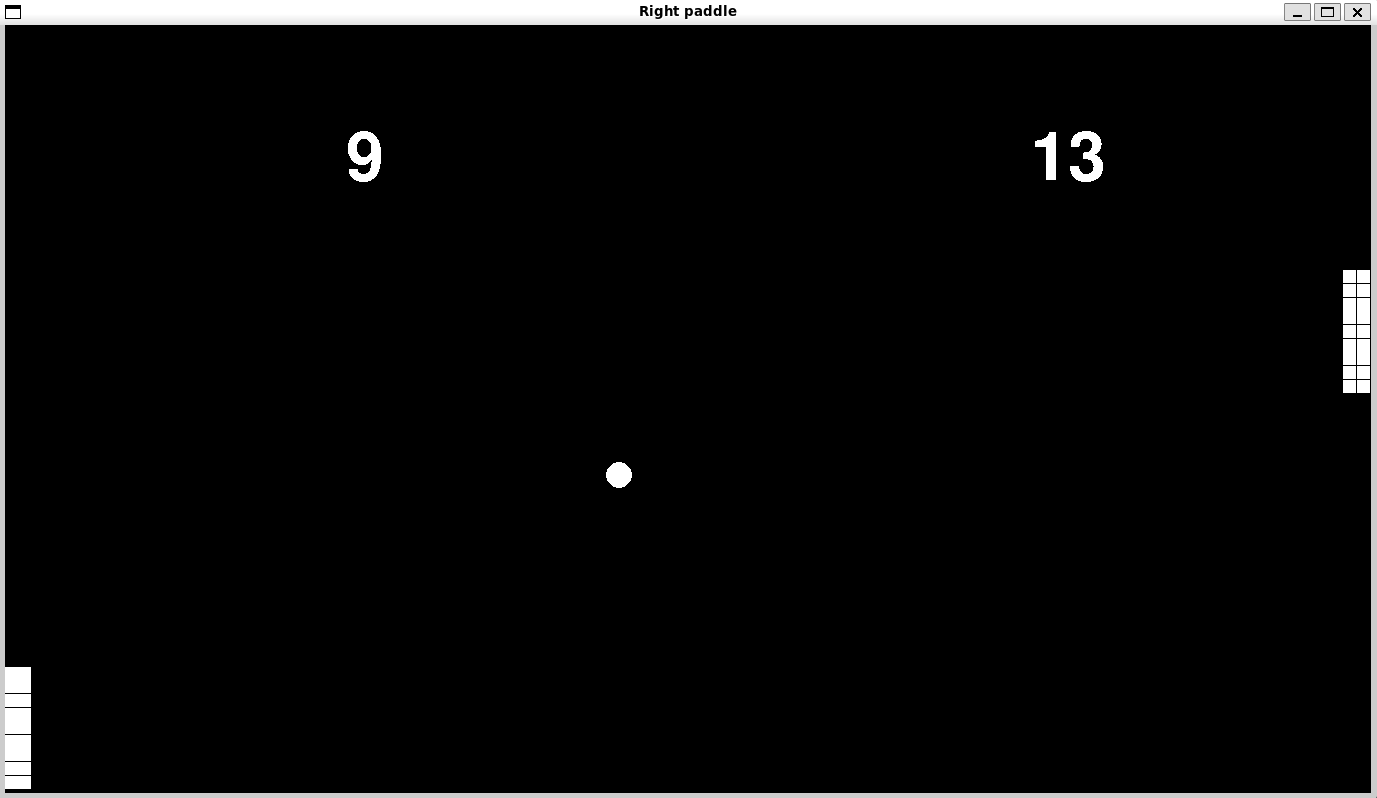
\includegraphics[scale=0.4]{img/gioco}
    \caption{Immagine dell'interfaccia di gioco}
    \label{fig:gioco}
\end{figure}

Il gioco viene avviato tramite linea di comando passando opzionalmente l'indirizzo dell'altro peer
(se questi non viene inserito, l'applicazione utilizza l'indirizzo di loopback). \\
Dopo aver passato gli argomenti ottenuti da linea di comando, il programma richiama la funzione \textit{peer\_run}
che è divisa in due parti:
\begin{itemize}
    \item \textbf{Creazione del peer e delle variabili di gioco} (Figura \ref{fig:inizializzazione})
    Vengono inizializzate tutte le variabili necessarie al funzionamento della partita, tra cui la griglia di gioco,
    la classe del peer locale e le variabili necessarie al funzionamento di \textit{pygame}
    \item \textbf{Il game loop} (Figura \ref{fig:game-loop}), ovvero il loop del gioco vero e proprio, composto come segue:
    \begin{itemize}
        \item Ottenimento dell'input da parte dell'utente, il tasto W muove la racchetta verso l'alto, mentre il
        tasto S la muove verso il basso.
        \item Invio del pacchetto UDP contenente le informazioni sulla propria racchetta e ricezione del pacchetto
        della controparte.
        \item A questo punto, il seeder gestisce opportunamente il movimento della pallina, se la pallina esce
        da un lato della griglia, procede ad aggiornare opportunamente lo scorekeeper, e invia i dati alla controparte. \\
        Nel mentre l'altro peer si limita ad ottenere i dati dalla controparte.
        \item Infine, entrambi i peer aggiornano la propria griglia in base ai dati posseduti e aggiornano il display.
    \end{itemize}
\end{itemize}

\begin{figure}
    \begin{verbatim}
        # Import omessi per semplicità

        def peer_run(args):
            # inizializzazione delle variabili
            grid = Grid()
            pygame.init()
            pygame.font.init()
            screen = pygame.display.set_mode((SCREEN_WIDTH, SCREEN_HEIGHT))
            clock = pygame.time.Clock()

            # creazione del peeer
            peer = Peer(args.peer_id)
            peer.set_other_peer(args.other_peer_address)

            # LEFT_PADDLE_ID è 0
            if peer.id == LEFT_PADDLE_ID:
                pygame.display.set_caption("Left paddle")
            else:
                pygame.display.set_caption("Right paddle")

            # continua...
    \end{verbatim}
    \caption{Inizializzazione del gioco}
    \label{fig:inizializzazione}
\end{figure}

\begin{figure}
    \begin{verbatim}
        # main game loop
        # alcune parti omesse per semplicità
        while True:
            # gestione dell'input
                # se viene premuto W...
                peer.controlled_paddle.velocity = -1
                # se viene premuto S...
                peer.controlled_paddle.velocity = 1

            # scambio dei dati delle proprie racchette
            peer.controlled_paddle.move()
            peer.send_data(peer.controlled_paddle)
            peer.receive_and_replace_object_data()

            if peer.ball.seeder_id == peer.id:
                # la pallina viene mossa oportunamente
                # e la posizione aggiornata viene inviata
                peer.send_data(peer.ball)
                if peer.ball.is_out():
                    if peer.ball.pos_x <= 0:
                        peer.scorekeeper.add_score(left_paddle_scored=False)
                    elif peer.ball.pos_x >= GRID_WIDTH:
                        peer.scorekeeper.add_score(left_paddle_scored=True)
                    peer.ball.reset_position()
                    peer.ball.set_random_velocity()
                    peer.send_data(peer.ball)
                    peer.send_data(peer.scorekeeper)
            # l'altro peer ottiene semplicemente i dati
            else:
                peer.receive_and_replace_object_data()
                peer.receive_and_replace_object_data()

            # aggiornamento della griglia,
            # del codice è stato omesso per semplicità
            grid.update_grid(  # args  )
            grid.display(screen)
            peer.scorekeeper.display(screen)
            pygame.display.flip()
            clock.tick(FPS)
    \end{verbatim}
    \caption{Il game loop}
    \label{fig:game-loop}
\end{figure}

    %! Author = Raffaele
%! Date = 17/01/2024

\thispagestyle{headings}
\newpage
\section{Manuale istruzioni sull'esecuzione}\label{sec:istruzioni}
\textit{Assicurarsi di avere Python installato su ogni macchina, il progetto è stato sviluppato con Python 3.11.4} \\ \\
L'applicazione può essere eseguita come segue:
\begin{itemize}
    \item Clonare la repository:
        \begin{verbatim}
            git clone
            https://github.com/rt2013G/reti9-network-pong.git
            && cd reti9-network-pong
        \end{verbatim}
    \item Creare un virtual environment ed attivarlo:
        \begin{verbatim}
            virtualenv -p python3 ./venv
            && source ./venv/bin/activate
        \end{verbatim}
    \item Installare i package necessari:
        \begin{verbatim}
            pip install -r requirements.txt
        \end{verbatim}
    \item Avviare l'applicazione sulla macchina su cui utilizzare la racchetta di \textbf{destra}. \\
    Questo passaggio è importante in quanto di default il seeder iniziale è la racchetta sinistra. \\
        \begin{verbatim}
            python3 pong.py 1 <IP controparte>
        \end{verbatim}
        oppure, se i due processi si trovano sulla stessa macchina:
        \begin{verbatim}
            python3 pong.py 1
        \end{verbatim}
        L'applicazione inserirà automaticamente l'indirizzo di loopback in questo caso.
    \item Avviare l'applicazione sulla macchina su cui utilizzare la racchetta di \textbf{sinistra}. \\
    Attenzione: il gioco inizierà automaticamente
        \begin{verbatim}
            python3 pong.py 0 <IP controparte>
        \end{verbatim}
        oppure, se i due processi si trovano sulla stessa macchina:
        \begin{verbatim}
            python3 pong.py 0
        \end{verbatim}
        L'applicazione inserirà automaticamente l'indirizzo di loopback in questo caso.
\end{itemize}


    \newpage
    \pagestyle{plain}

\end{document}